\chapter{Data Preprocessing}

\section{Data Cleaning}

With \texttt{RStudio}, the working directory is automatically determined. Otherwise, it can be indicated by \texttt{here} library.

\begin{lstlisting}[caption={Required libraries and working directory setup}]
  # Libraries and options
  library(dplyr)
  library(here)
  library(knitr)
  library(kableExtra)
  
  # Self-defined functions
  source("utils.R")
  
  # Working directory
  setwd(here())
  \end{lstlisting}

Now our working directory have been explicated, we can use relative paths to read the data. With \texttt{RMarkdown}, we can prettify the rendering.

\begin{lstlisting}[caption={RStudio data object initialization}]
    # Read the CSV file into a data frame
    cpu_data <- read.csv("dataset/Intel_CPUs.csv")
    gpu_data <- read.csv("dataset/All_GPUs.csv")
    
    # Inspect the CPU data
    kable(head(cpu_data), format = "html") %>%
      kable_styling()
    \end{lstlisting}

\begin{figure}[!ht]
  \centering
  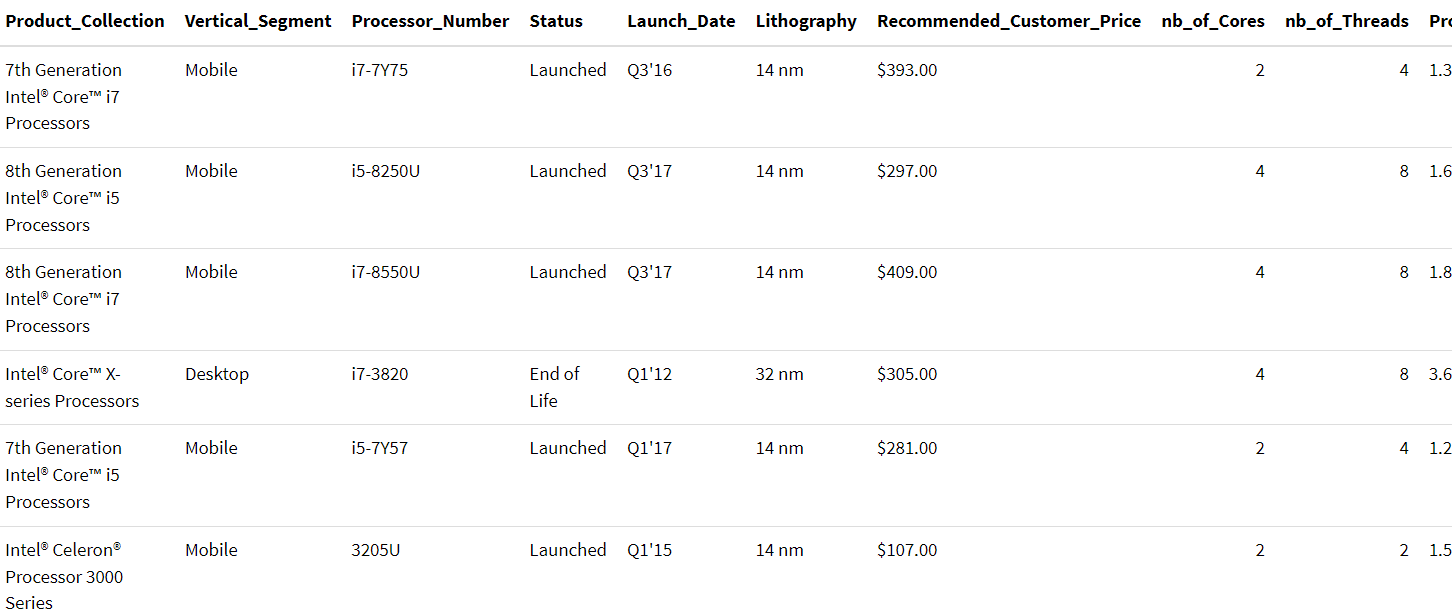
\includegraphics[width=\textwidth]{img/cpu-head.png}
  \vspace{0.5cm}
  \caption{First instances of CPUs data}
\end{figure}

Invalid cells may contain \texttt{NA}, an empty string, or other values showing us that this cell's data was not collecting correctly. At the very first step, we want to select only columns such that the percentage of valid cells exceeds our predefined value. Then we filter out all instances with invalid features. Note that careful column selection possibly remains more instances for later tasks. For CPU data, we concern about the price, so let us choose a quota for which the column of prices is maintained.

\begin{lstlisting}[caption={Cleaning functions}]
  # Check if a cell has a valid value
  is_valid <- function(value) {
    return(!is.na(value)
           & !is.null(value)
           & !value == ""
           & !value == "N/A"
           & !trimws(value) == "-"
           & !value == "missing"
           & !value == "unknown")
    # Add your criteria
  }
  
  
  # Select columns with enough valid cells
  filtered_data <- function(data, valid_percentage=0.5) {
  selected_columns <- character(0) 
  
  for (col in colnames(data)) { 
    valid_count <- sum(is_valid(data[[col]])) 
    total_instances <- length(data[[col]]) 
    
    if ((valid_count / total_instances) >= fill) {
      selected_columns <- c(selected_columns, col)
    }
  }
  
  return(data[selected_columns])
}
  \end{lstlisting}


\begin{lstlisting}[caption={Cleaned CPU data}]
  filtered_cpu_data <- filtered_data(cpu_data, valid_percentage=0.5)

  processed_cpu_data <- 
    filtered_cpu_data[
      apply(filtered_cpu_data, 1, function(row) all(sapply(row, is_valid))), ]
  
  selected_cpu_data <- processed_cpu_data[] # Adjust selected columns for your later needs
  selected_cpu_data <- unique(selected_cpu_data)
  kable(head(selected_cpu_data), format = "html") %>%
    kable_styling()
\end{lstlisting}

\begin{lstlisting}[caption={Cleaned GPU data}]
  filtered_gpu_data <- filtered_data(gpu_data, valid_percentage=0.5)

  processed_gpu_data <- 
    filtered_gpu_data[
      apply(filtered_gpu_data, 1, function(row) all(sapply(row, is_valid))), ]
  
  selected_gpu_data <- processed_gpu_data[] # Adjust selected columns for your later needs
  selected_gpu_data <- unique(selected_gpu_data)
  kable(head(selected_gpu_data), format = "html") %>%
    kable_styling()
\end{lstlisting}

\begin{figure}[!ht]
  \centering
  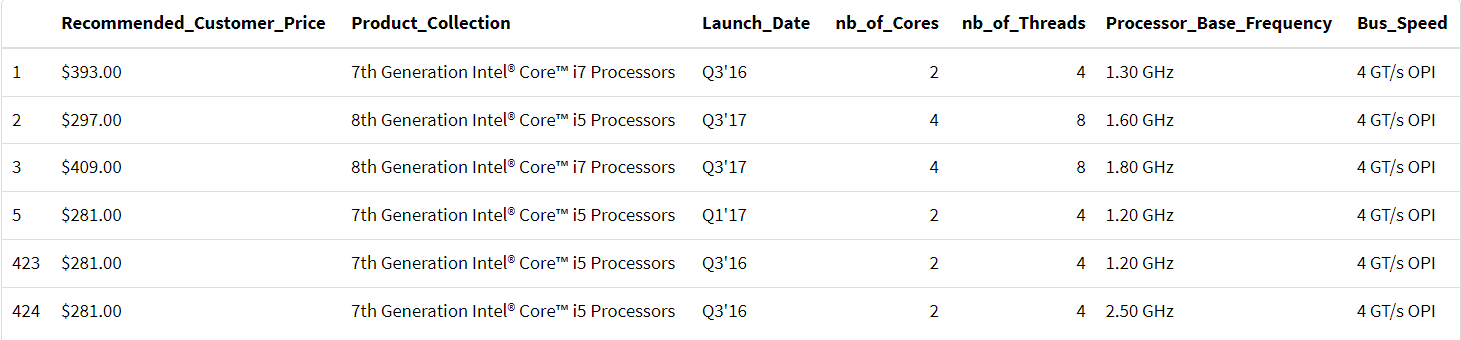
\includegraphics[width=\textwidth]{img/cpu-selected-head.png}
  \vspace{0.5cm}
  \caption{First instances of selected CPUs data}
\end{figure}

\begin{figure}[!ht]
  \centering
  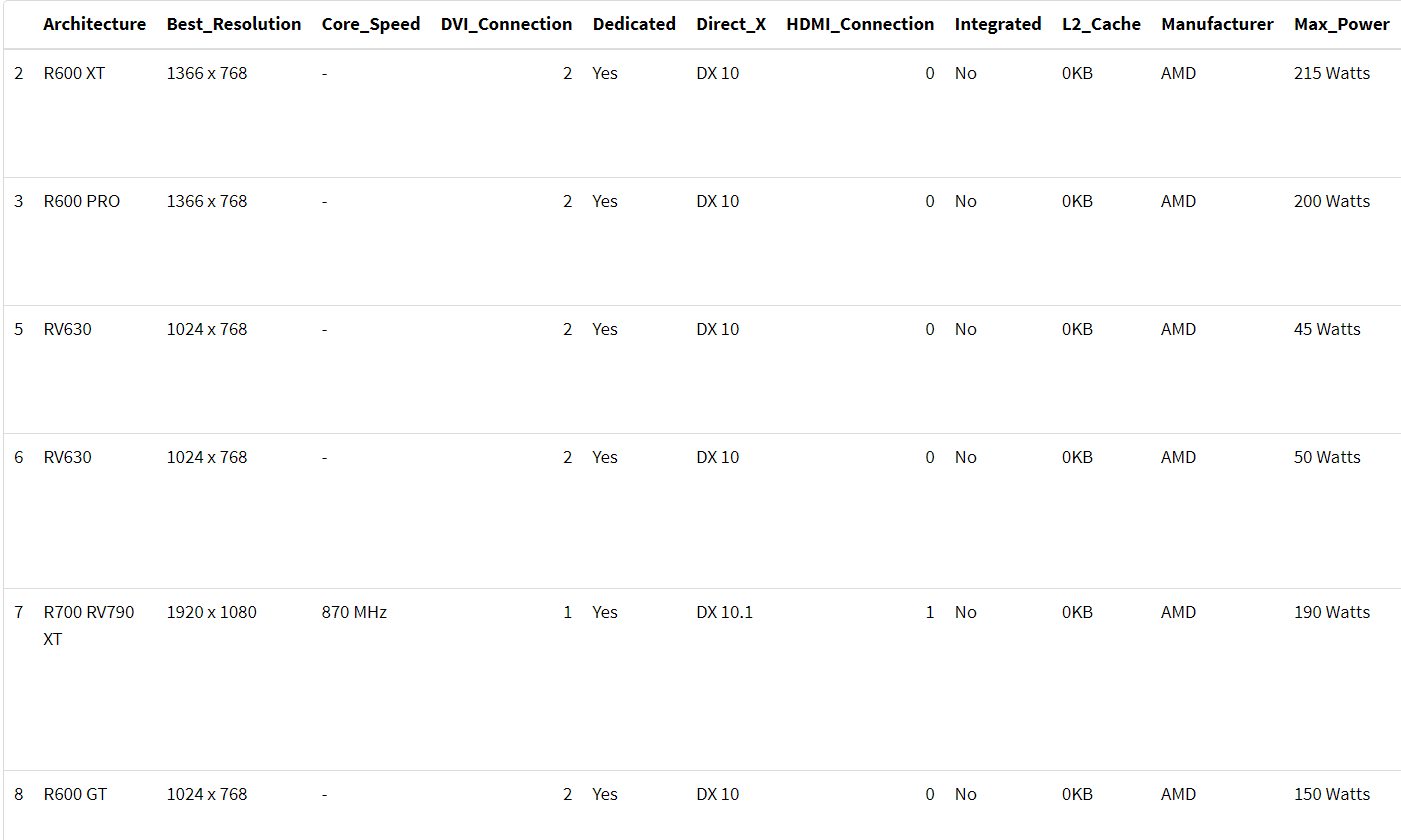
\includegraphics[width=\textwidth]{img/gpu-selected-head.png}
  \vspace{0.5cm}
  \caption{First instances of selected GPUs data}
\end{figure}

It's worth finding the key of the data to know which feature uniquely determine an instance. We prioritize categorical features, specifically pure names.

\begin{lstlisting}[caption={Keys of the data}]
  nrow(selected_cpu_data) - nrow(selected_cpu_data[, c("Product_Collection", 
                                                       "Processor_Number")])
  nrow(selected_gpu_data) - nrow(selected_gpu_data[, c("Name")])
  # Outputs: 0
\end{lstlisting}


\section{Data Pre-computation}

Some features in our data have values that need to be reformatted for easily later sorting and analyses. Therefore, we need to gain a good understand on the features.


\begin{lstlisting}[caption={A processing for selected features}]
  cpu_columns <- colnames(cpu_data)
  gpu_columns <- colnames(gpu_data)
  intersect(cpu_columns, gpu_columns)
  # Output: character(0)
\end{lstlisting}

Since the data files have no common features, we took a look at them independently and decided to pre-compute some features.

\begin{enumerate}
  \item Use the common column name \texttt{Release\_Date} for both data. Extract \texttt{Release\_Year} and \texttt{Release\_Quarter} for each instance.
  \item If \texttt{Recommended\_Customer\_Price} is a range, compute the average.
\end{enumerate}

\begin{lstlisting}[caption={Extract Year and Quarter from Dates}]
  month_to_quarter <- function(month) {
  quarter <- switch(month,
                    "Jan" = "1",
                    "Feb" = "1",
                    "Mar" = "1",
                    "Apr" = "2",
                    "May" = "2",
                    "Jun" = "2",
                    "Jul" = "3",
                    "Aug" = "3",
                    "Sep" = "3",
                    "Oct" = "4",
                    "Nov" = "4",
                    "Dec" = "4",
                    "Unknown")
  return(quarter)
}

names(selected_cpu_data)[names(selected_cpu_data) == "Launch_Date"] <- "Release_Date"
selected_cpu_data$Release_Year <- as.integer(sub("Q[1-4]'(\\d+)", "\\1", 
                                             gsub("\\s+", "", selected_cpu_data$Release_Date))) + 2000
selected_cpu_data$Release_Quarter <- as.integer(sub("Q([1-4])'.*", "\\1", 
                                                gsub("\\s+", "", selected_cpu_data$Release_Date)))

selected_gpu_data$Release_Year <- 
  as.integer(sub(".*-(\\d{4}) .*", "\\1", selected_gpu_data$Release_Date))
selected_gpu_data$Release_Quarter <- 
  as.character(sub(".*-(\\w+)-\\d{4}.*", "\\1", selected_gpu_data$Release_Date))
selected_gpu_data$Release_Quarter <- sapply(selected_gpu_data$Release_Quarter, month_to_quarter)
\end{lstlisting}